\subsection{Hardware Design}
\label{sec:des-hardware}
\subsubsection{Plotter designs and mechanics}
The chosen method of text plotting is a Cartesian gantry system with 2 independent axes of movement with a pen up/down mechanicsm. Complex kinematics equations and error dependencies are avoiding by using 2 isolated x and y movement methods for reproduction \cite{teikari2016}. Linear GT2 timing belts and pulleys are used to convert rotary motion from stepper motors and axles to the desired cartesian movements. Timing belts are used for their reliability, cost effectiveness, and higher speed travel \cite{iqs2024}.

A Cartesian gantry consists of a stationary rail that controls movement in one axis, and a movable rail that controls the other axis of movement. For this system and future explanations, the stationary rails control y-axis movement, while the x-axis rail moves along the y-axis. Figure~\ref{fig:gantry-axis-diagram} shows the fixed rails guiding $y$ movement, the moving $x$ rail and the separate pen lift.

\begin{figure}[H]
    \centering
    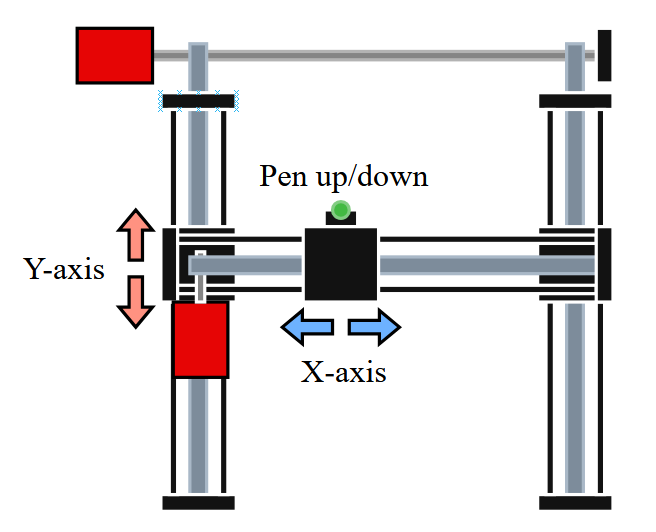
\includegraphics[width=0.72\linewidth]{Figures/gantry-axis-diagram.png}
    \caption{Cartesian gantry axes and pen up/down mechanism.}
    \label{fig:gantry-axis-diagram}\label{fig:des-gantry-axes}
\end{figure}

The x-axis rail needs to move with stability and consistency, which is why it is supported on both ends by dual-rails on the y-axis. A singular stepper motor was chosen to drive both pulleys on both y-axis rails to ensure synchronicity and save costs. 2 independent stepper motors driving one axis creates synchronicity issues because any difference in timing, missed steps or load torques could offset the movement between the two motors. The challenge with using one motor to drive two timing pulleys, is finding a method to extend the shaft of the motor to connect to both timing pulleys without overloading the motor and applying too much tortion or twist to the new axle. A rigid coupler was used to extend the axle of the stepper motor to a chromed steel rod.

To reduce strain on motors, and allow for increased accuracy and precision, linear bearing were fitted around the chromed rod rails to allow all parts to slide with very little friction.
To verify the stepper motor could handle the weight of the x-axis rail further, the torque required to move the rail at the desired speed was calculated. It is described in Section 3.3.2 with the descriptions of the stepper motor type chosen and its product specifications.


All CAD models for this project were designed from first principles using Autodesk Fusion360, with no off the shelf housings used, including all designs for the gantry system as well as the camera housing module. Designs were created by identifying off-the-shelf hardware components that were available and had to be acquired, and designing around these components with decent tolerances to allow for easy contruction and precision.

The three pen-lift parts in Figure~\ref{fig:gantry-cad-pen} work together: the cam rotates by 90 degrees at a time to control the lift, while the mounting pieces hold the pen in position relative to its up/down state, with springs constantly applying a downward pressure to act as dynamic pen pressure control.

\begin{figure}[H]
    \centering
    \begin{minipage}[c]{0.32\linewidth}
        \centering
        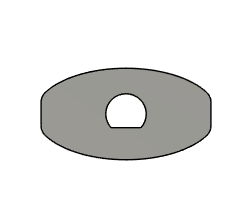
\includegraphics[width=\linewidth,height=0.16\textheight,keepaspectratio]{Figures/cad-component-01.png}\par(a)
    \end{minipage}\hfill
    \begin{minipage}[c]{0.32\linewidth}
        \centering
        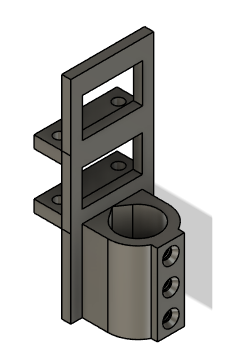
\includegraphics[width=\linewidth,height=0.16\textheight,keepaspectratio]{Figures/cad-component-02.png}\par(b)
    \end{minipage}\hfill
    \begin{minipage}[c]{0.32\linewidth}
        \centering
        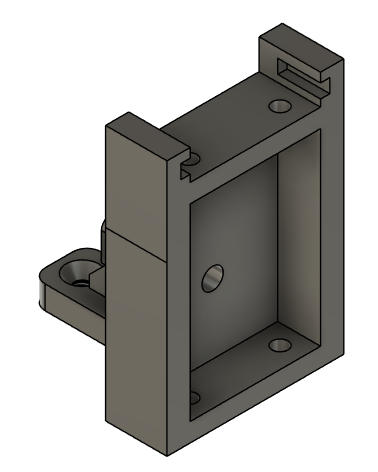
\includegraphics[width=\linewidth,height=0.16\textheight,keepaspectratio]{Figures/cad-component-03.png}\par(c)
    \end{minipage}
    \caption{CAD models of the cam and pen-mounting parts.}
    \label{fig:gantry-cad-pen}
\end{figure}

Figures~\ref{fig:gantry-cad-brackets} and~\ref{fig:gantry-cad-belt} show the different mounting part used for the drive chain, used to hold the timing belt pulleys as well as the stepper motor in place. Chamfered threaded screw holes are added so the design maybe be screwed fastly into the correctly position on the base with M4 bolts.

\begin{figure}[H]
    \centering
    \begin{minipage}[c]{0.48\linewidth}
        \centering
        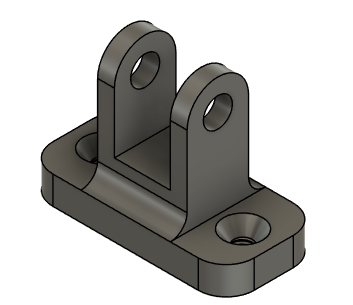
\includegraphics[width=\linewidth,height=0.16\textheight,keepaspectratio]{Figures/cad-component-04.png}\par(d)
    \end{minipage}\hfill
    \begin{minipage}[c]{0.48\linewidth}
        \centering
        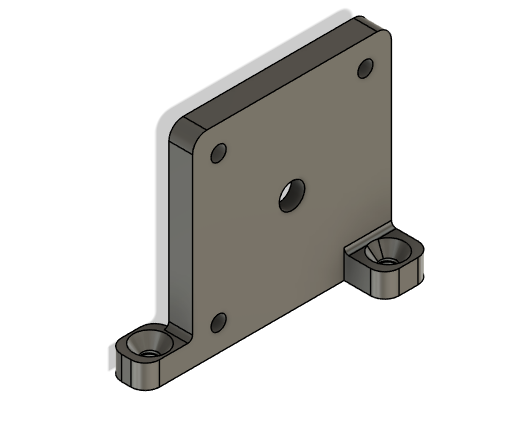
\includegraphics[width=\linewidth,height=0.16\textheight,keepaspectratio]{Figures/cad-component-05.png}\par(e)
    \end{minipage}
    \caption{CAD models of the drive support brackets.}
    \label{fig:gantry-cad-brackets}
\end{figure}

The toothed belt grip shown in Figure~\ref{fig:gantry-cad-belt} secures the belt to the moving assembly, transferring belt motion to the gantry. It is designed to be removable and adjustable to allow for tightening or loosening of the timing belt.

\begin{figure}[H]
    \centering
    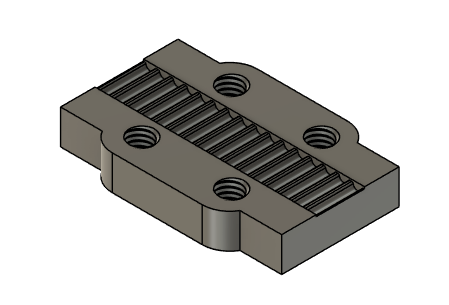
\includegraphics[width=0.48\linewidth,height=0.16\textheight,keepaspectratio]{Figures/cad-component-06.png}\par(f)
    \caption{CAD model of the toothed-belt grip.}
    \label{fig:gantry-cad-belt}
\end{figure}

The bearing and rod supports in Figure~\ref{fig:gantry-cad-guides} locate the rails and guide the moving parts along them.

\begin{figure}[H]
    \centering
    \begin{minipage}[c]{0.48\linewidth}
        \centering
        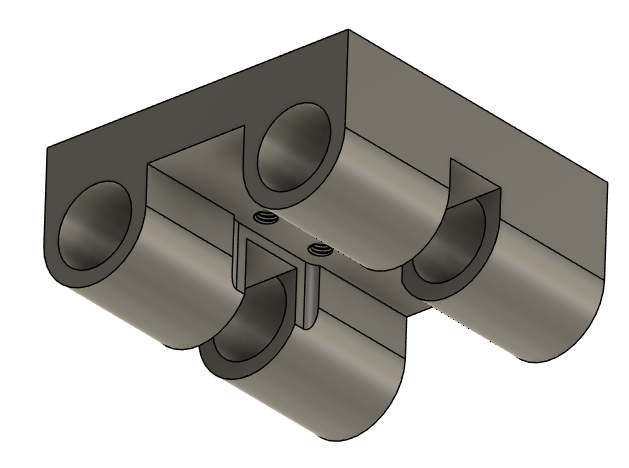
\includegraphics[width=\linewidth,height=0.16\textheight,keepaspectratio]{Figures/cad-component-07.png}\par(g)
    \end{minipage}\hfill
    \begin{minipage}[c]{0.48\linewidth}
        \centering
        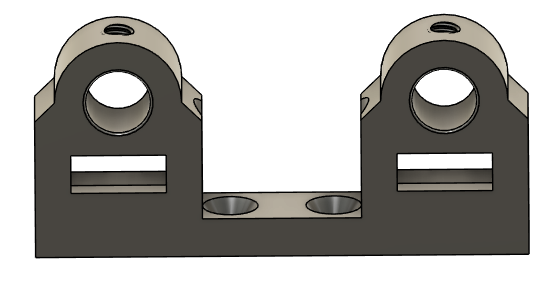
\includegraphics[width=\linewidth,height=0.16\textheight,keepaspectratio]{Figures/cad-component-08.png}\par(h)
    \end{minipage}
    \caption{CAD models of the bearing and rod supports.}
    \label{fig:gantry-cad-guides}
\end{figure}

\label{sec:des-camera}
The camera housing was designed to hold the IMX179 USB webcam module securely. Its single curved supporting arm is intended to reduce shadows on the page. Page clamps hold each page securely in place to minimise rotation and skew errors. Figure~\ref{fig:camera-cad} shows the camera housing and page-clamp designs; panel~(a) shows the assembled housing and clamps, and panel~(b) shows the camera housing plate that slots into the support structure.

\begin{figure}[H]
    \centering
    \begin{minipage}[t]{0.48\linewidth}
        \centering
        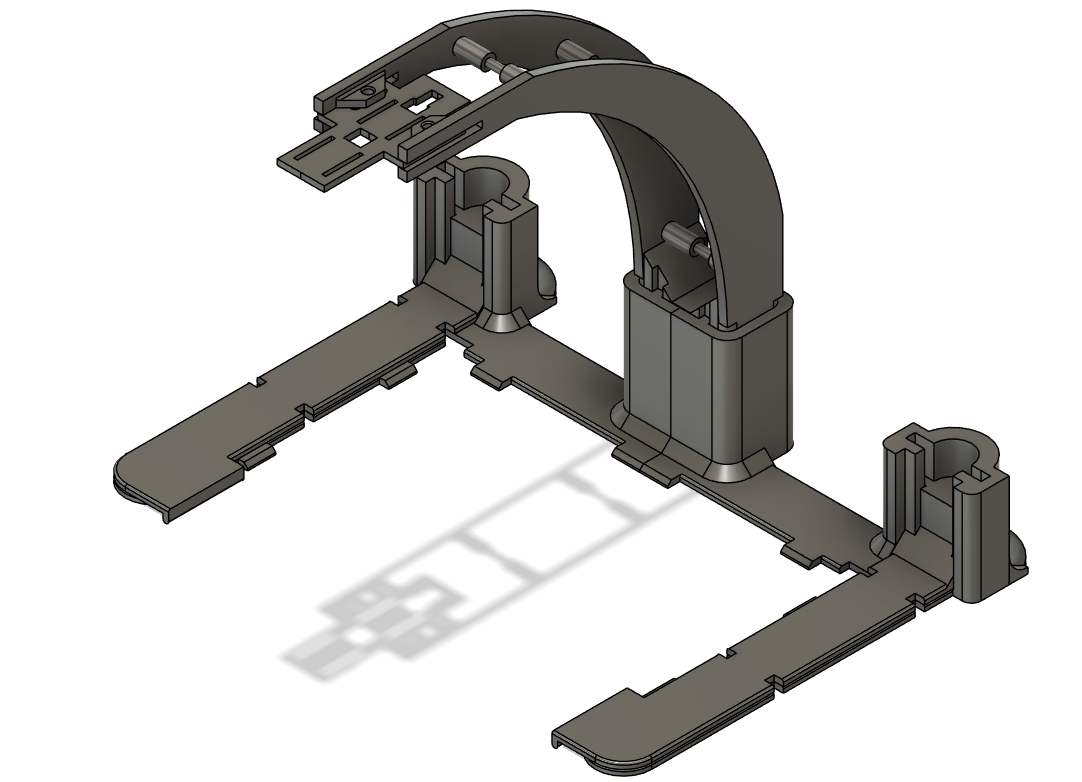
\includegraphics[width=\linewidth,height=0.25\textheight,keepaspectratio]{Figures/camera-housing-assembly.png}
        \par\smallskip\small (a) Camera housing, curved support arm and page clamps.
    \end{minipage}\hfill
    \begin{minipage}[t]{0.48\linewidth}
        \centering
        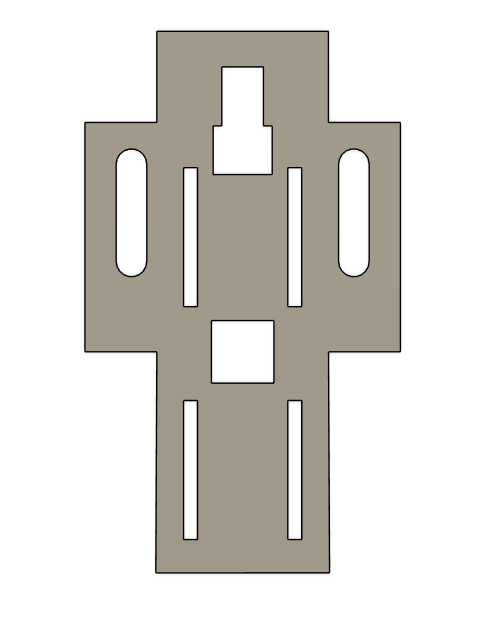
\includegraphics[width=\linewidth,height=0.25\textheight,keepaspectratio]{Figures/camera-page-clamp.png}
        \par\smallskip\small (b) Page-clamp component.
    \end{minipage}
    \caption{CAD designs for the camera housing and page clamps.}
    \label{fig:camera-cad}
\end{figure}


\subsubsection{Stepper motor and driver}
\label{sec:des-stepper}
A stepper motor does not continuously turn with a PWM input, but rather turns at specific fixed angles each time there is a switch in the windings (the coils of the stepper motor). The A4988 regulates the winding current through a process called chopping, which switches the current supply on the winding until the current rises to a certain point, and then switches off at the target current.  This occurs at high frequencies and effectively keeps the current going to the coils within a specific range so as to not overshoot, even when the motor is not actively stepping. A step is created by slighty adjusting the current value between 2 coils just enough to allow the rotors teeth to make a small jump or 'step'. The stepper motor is perfect for the precise movements required for handwriting reproduction with the gantry, as it produces steps at exact, known intervals, with position tracked from commanded steps rather than an encoder. This assumes that the motors do not miss steps. 

Two stepper motors are used in the gantry plotter, one for x and one for the y-axis direction. The type of stepper motor chosen was the 42BYGH40-01 Nema 17 bipolar stepper motor, with a resolution of 200 full steps per revolution and a current rating of 1.68A per phase~\cite{stepperds}. 

The following calculations were done to determine if the Nema 17 stepper motor would be strong enough for the use case of the gantry plotter, and if a singular motor could control both y-axis belt drives safely.

Dziedzic et al. examined samples written at 10--60\,mm/s~\cite{dziedzic2026}. The maximum handwriting speed mentioned was 3600mm/min, which was rounded up to 4000mm/min for headroom and approximately 10\% tolerance. 

For the 20-tooth GT2 pulleys with 2mm belt pitch that were used for the gantry, the belt travel during one rotation is calculated as follows gives~\cite{acarnley2002}
\begin{equation}
\ell_{\mathrm{rev}}=N_t p=20(2)=40\ \mathrm{mm/rev},\qquad
r_p=\frac{N_t p}{2\pi}=6.37\ \mathrm{mm}.
\label{eq:des-pulley}
\end{equation}
$N_t$ refers to the number of teeth on the pulley, $p$ is the belt pitch, and $\ell_{\mathrm{rev}}$ is the belt travel during one full pulley revolution. The pitch radius $r_p$ is the effective radius of the belt path around the pulley.

\paragraph{Speed-to-torque margin check.}
The chosen max gantry speed to achieve is converted to a motor speed and compared with the torque required to move the assembly. 

\begin{equation}
n = \frac{v}{\ell_{\mathrm{rev}}} = \frac{4000\ \mathrm{mm/min}}{40\ \mathrm{mm/rev}} = 100\ \mathrm{RPM}
\label{eq:gan-rpm}
\end{equation}

where $n$ is the motor speed in revolutions per minute, $v=4000$\,mm/min is the max gantry speed decided upon as previously mentioned, and $\ell_{\mathrm{rev}}=40$\,mm is the belt travel per revolution previously calculated. To then calculate the pull-out torque the system experiences at this speed, interpolation is done on the NEMA 17 pull-out torque curve found in SOURCE
\begin{equation}
T_{\mathrm{po}}(n) = T_1 + \frac{n-n_1}{n_2-n_1}\bigl(T_2-T_1\bigr) = 7 + \frac{100-60}{120-60}(21-7) \approx 16.3\ \mathrm{N\,cm}
\label{eq:gan-pullout}
\end{equation}

where $T_{\mathrm{po}}(n)$ is the interpolated pull-out torque estimate at speed $n$, and the measured curve readings are $(60\ \mathrm{RPM},\,7\ \mathrm{N\,cm})$ and $(120\ \mathrm{RPM},\,21\ \mathrm{N\,cm})$. 

To then calculate the torque required at constant velocity, the following formula and calculation is done, based off of bearing friction, mass, and the previously calculated effective radius of the belt path. SOURCE
\begin{equation}
T_{\mathrm{req}} = r\,F_f = r\,\mu\,m\,g = 0.006366 \times 0.004 \times 0.950 \times 9.81 \approx 0.0237\ \mathrm{N\,cm}
\label{eq:des-torque}
\end{equation}

where $T_{\mathrm{req}}$ is the torque needed at constant velocity, $r=6.37$\,mm is the pulley pitch radius , $\mu=0.004$ is the original assumed bearing-friction coefficient, $m=0.950$\,kg is the complete moving assembly and $g=9.81$\,m/s$^2$. 

The calculated torque needed at constant velocity to move the 0.95kg x-rail, is only $0.0237\ \mathrm{N\,cm}$, which is significantly lower than the interpolated pull-out torque of the NEMA stepper motor at the maximum use case travelsal speed. (16.3N)

Figure~\ref{fig:stepper-motor-and-driver} shows the selected motor and its A4988 driver.

\begin{figure}[H]
    \centering
    \begin{minipage}[c]{0.48\linewidth}
        \centering
        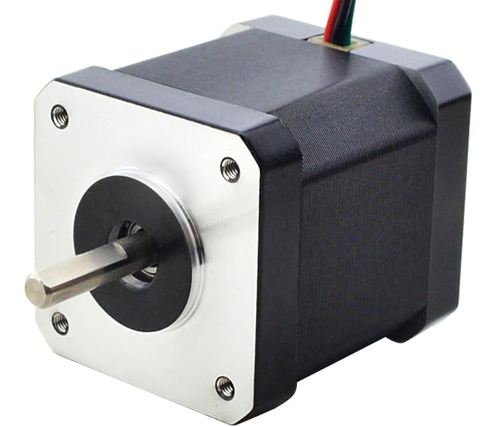
\includegraphics[width=\linewidth,height=0.2\textheight,keepaspectratio]{Figures/nema-17-stepper-motor.png}
    \end{minipage}\hfill
    \begin{minipage}[c]{0.48\linewidth}
        \centering
        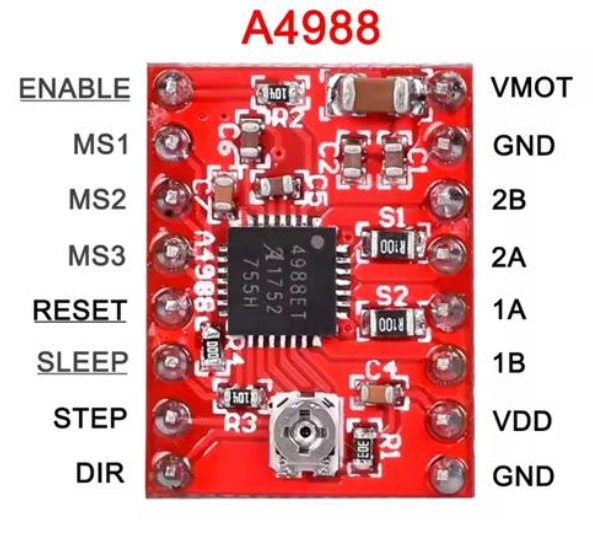
\includegraphics[width=\linewidth,height=0.2\textheight,keepaspectratio]{Figures/a4988-stepper-driver.png}
    \end{minipage}
    \caption{NEMA 17 motor and A4988 driver.}
    \label{fig:stepper-motor-and-driver}
\end{figure}

\subsubsection{Step resolution, microstepping and calibration}
\label{sec:gan-res}
\label{sec:gan-timing}

Three properties of a stepper drive fix the resolution of this machine. The motors used here take 200 full steps per revolution, so one full step is $1.8^\circ$; because position is simply the number of steps that the motor was signlalled to produce, with no encoder or feedback loop required to verify this due to the consistent nature of the stepper motors. The driver subdivides each full step by microstepping: rather than switching the two windings fully on or off, it holds them at intermediate current ratios, placing the rotor at intermediate angles in the stepper motor. At the 1/16 setting on the driver, one full step becomes 16 microsteps, so a revolution is 3200 microsteps. This maximum microstepping option was used for this project because it has increased resolution and smoother motion. The only downside is that at higher load torques, steps could slip due to the intermediary position of the motors.

The following equations are used to determine if the stepper motor resolution will be fine enough to fulfill the 0.5mm gantry precision tolerance requirement specified in the project proposal. Equation~\ref{eq:des-stepres} gives the step resolution from 200 full steps~\cite{stepperds}, 16 microsteps~\cite[p.~6]{a4988ds} and $\ell_{\mathrm{rev}}=40$\,mm,
\begin{equation}
K=\frac{200\cdot16}{\ell_{\mathrm{rev}}}=\frac{3200}{40}=80\ \mathrm{steps/mm},\qquad\Delta=\frac1K=12.5\ \mu\mathrm{m},
\label{eq:des-stepres}
\end{equation}
where K is the steps/mm resolution of the stepper motor driver, and $\Delta$ is interval step size of the stepper motor. The  Quantisation error is at most $\Delta/2=6.25\ \mu$m per axis, $8.8\ \mu$m combined over both axes as a pythagorean measurement, which is significantly smaller than the 0.5mm tolerance of R5. Multiple other factors could still affect the gantry precision including belt stretch, backlash, missed steps, switch repeatability and flexibility in the pen housing.
\paragraph{Coil current and its derating.}
To calculate the appropriate $V_{\mathrm{ref}}$ to set with the potentiometer on the A4988 stepper motor driver, the datasheet relation~\cite[p.~9]{a4988ds} between the the carrier's two sense resistors and the regulated current of the stepper motor and driver gives
\begin{equation}
I_{\mathrm{coil}}=\frac{V_{\mathrm{ref}}}{8\,R_S}\quad, \quad V_{\mathrm{ref}}=8\,R_S\,I_{\mathrm{coil}}=8\cdot0.1\cdot1.68=1.34\ \mathrm{V}
\label{eq:des-current}
\end{equation}
for the 1.68\,A motor rating~\cite{stepperds}, conditional on the R10 sense-resistor marking meaning $0.1\,\Omega$. This gives gives the safe maximum operating $V_{\mathrm{ref}}$ for the system to operate at, and the potentiometer on the A4988 stepper motor driver was tweaked to match the $V_{\mathrm{ref}}$.

\subsubsection{Pen up/down mechanism}
\label{sec:des-pen}\label{sec:gan-circuits}\label{sec:des-power}
The pen-lift mechanism itself is a design choice justified against the alternative of a third stepper or a servo motor. A servo motor expects a continuous pulse-width-modulated position command and typically needs its own timer a precisely timed software loop running concurrently with the gantry's own step timing, competing for the same processor cycles that generate STEP pulses. An N20 geared d.c.\ motor run in one direction only, with a cam that toggles the pen up or down every $90^\circ$ of rotation, needs only an on/off drive pulse of roughly known duration and a microswitch to act as the feedback loop to verify the pen up position. It is cheap, widely available, has high torque at low speed because of its internal gearbox, has an incredibly small profile, and has no accuracy or positioning cost due to the use of a switch for the feedback loop.

Figure~\ref{fig:pen-up-down-mechanism} shows the cam holding the pen in its two positions.

\begin{figure}[H]
    \centering
    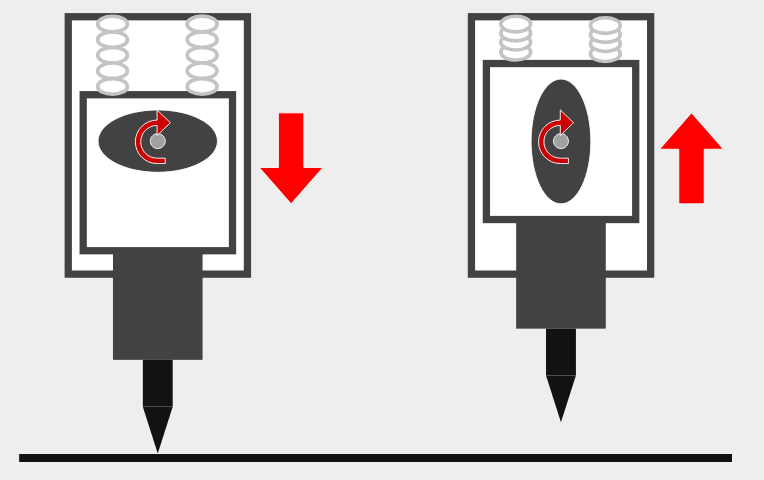
\includegraphics[width=0.75\linewidth]{Figures/pen-up-down-mechanism.png}
    \caption{Pen lowered (left) and raised (right).}
    \label{fig:pen-up-down-mechanism}\label{fig:des-penmechanism}
\end{figure}

The implemented lift, planned in the proposal as a stepper, gives only pulses, so the pen state must be tracked in software, and the pen switch is feedback only (high = up). The pen-drive routine of Algorithm~\ref{alg:gan-pen} must therefore test the switch before energising the motor, since the cam turns one way only and an unnecessary pulse would toggle the pen to the wrong state rather than leave it alone. The controller runs the motor until the requested switch state is confirmed or a timeout occurs, with a 40ms overrun after pen-up confirmation. The generator's separate settling dwell is 350ms default setting, done through visual verification to make sure the pen was at its highest state when the up command was triggered.

\paragraph{Pen motor driver and base-resistor selection.}
The GA12-N20 geared motor was selected to turn the pen cam with a compact, low-speed geared output. The listed 3\,V, 150\,rpm variant has a specified voltage range of 1.5--5\,V, a no-load current of 10\,mA, a rated current of 30\,mA, and a stall current of 230\,mA~\cite{ga12n20ds}. The supplied circuit uses the Odroid's 3.3\,V GPIO signal (max 4mA output SOURCE) to drive the base of a BC337 NPN transistor. The transistor is a low-side switch: motor current flows from the 3.3\,V DC motor rail, through the motor and collector-emitter path to the shared ground, while the GPIO supplies only base current~\cite{odroidn2ds}. The source symbol in the supplied diagram should therefore be read as a DC supply, not an AC source.

The stated 4\,mA maximum GPIO output current sets a \emph{minimum}, not a maximum, base-resistor value. Assuming a base-emitter voltage of approximately 0.7\,V, the minimum resistance is
\begin{equation}
R_{B,\min}=\frac{V_{\mathrm{GPIO}}-V_{BE}}{I_{\mathrm{GPIO,max}}}=\frac{3.3-0.7}{0.004}=650\,\Omega.
\label{eq:des-base-resistor-min}
\end{equation}
A standard 1\,k$\Omega$ resistor was selected, which is above this minimum. Its nominal GPIO/base current is

\begin{equation}
I_B = \frac{V_{\mathrm{GPIO}}-V_{BE}}{R_B} = \frac{3.3-0.7}{1000} \approx 2.6\,\mathrm{mA}.
\label{eq:des-basecurrent}
\end{equation}
The nominal 2.6\,mA base current is below the stated 4\,mA GPIO output limit. Using a forced gain of 10, as in the BC337 saturation test~\cite{bc337ds}, gives a conservative 26\,mA collector-current check. This is below the listed 30\,mA motor rating, so saturation at rated motor current is not established by the base-resistor calculation alone.


Figure~\ref{fig:des-pencircuit} shows the transistor circuitry, with connections to the motor that spins the pen mechanism, a 3.3V source, ground, and the GPIO pin of the ODROID N2+.

\begin{figure}[H]
    \centering
    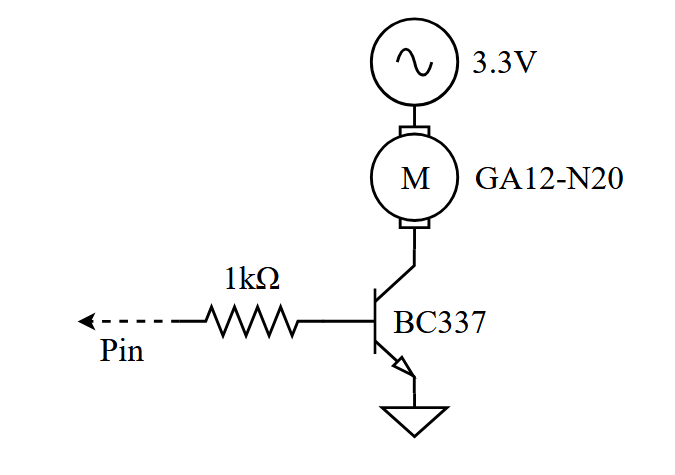
\includegraphics[width=0.5\linewidth]{Figures/pen-clicker-bc337-circuit.png}
    \caption{BC337 pen-motor switching circuit.}
    \label{fig:pen-clicker-bc337-circuit}\label{fig:des-pencircuit}
\end{figure}

\begin{algorithm}[!htbp]
\caption{Pen toggle}
\label{alg:gan-pen}
\begin{algorithmic}[1]
\REQUIRE desired state $\mathrm{wantUp}$
\IF{any end-stop is currently triggered}
    \STATE refuse the request
\ELSIF{the pen switch already reads $\mathrm{wantUp}$}
    \STATE \textbf{return} \COMMENT{the motor must \emph{not} run; the cam turns one way only}
\ELSE
    \STATE energise the pen motor
    \WHILE{before the deadline and the pen switch does not yet read go UP}
        \STATE wait
    \ENDWHILE
    \IF{the switch now reads up}
        \STATE wait 40\,ms more to seat the cam
    \ENDIF
    \STATE de-energise the pen motor
\ENDIF
\end{algorithmic}
\end{algorithm}

During tuning the clicker sometimes over-rotated and the pen did not push down fully before the switch read as triggered, requiring the switch timing to be adjusted experimentally. The pressure of the pen different surfaces like a soft clamp surfaces (exam pad) or a hard wooden base surface produced variations in the ink thickness, so a rigid clipboard with a single page clamped flat was decided to be used, for consistent pen pressures. 

\subsubsection{End stop switches and calibration}
\label{sec:des-calibration}
All four axis end-stop switches are checked before every major axis step, and every G-code line. Debouncing on the pen switches was imlemented digitally to ensure end-stops were never triggered from noise. A switch is only accepted to be triggered after three consecutive high reads 6\,ms apart (Algorithm~\ref{alg:gan-endstop}). The pen switch is read separately by the pen-control routine. 

The DML31P microswitch was selected as a compact lever microswitch for detecting gantry end-stop contact. It is as an SPDT (single-pole double throw) switch rated for 1\,A at 125\,V AC~\cite{dml31p}. In this circuit and for the use case of this project it is used only as a low-current logic contact detection, not to switch on a motor. The diagram uses the common and normally-open contacts so that actuating the switch connects the Odroid N2+'s 3.3\,V logic rail to the GPIO input; the source symbol represents DC. A standard 10\,k$\Omega$ resistor was a pull-down, to ensure the GPIO pin of the ODROID N2+ was provided with a current comfortably than the max 4mA the pin can handle ~\cite{odroidn2ds}. The circuit holds the input low while the switch is open, preventing a floating input, and draws a small current when the switch closes. 

With the switch closed, the pull-down current and resistor dissipation are, proving the current flowing through the system is significantly lower than the 4mA max of the GPIO pins, ensuring safety of the SBC.
\begin{equation}
I_{\mathrm{closed}}=\frac{V_{\mathrm{rail}}}{R_{\mathrm{PD}}}=\frac{3.3\,\mathrm{V}}{10\,\mathrm{k}\Omega}=0.33\,\mathrm{mA},\qquad
\label{eq:endswitch-pulldown}
\end{equation}

Figure~\ref{fig:des-switch} shows the switch contact and pull-down that define the GPIO input state.

\begin{figure}[H]
    \centering
    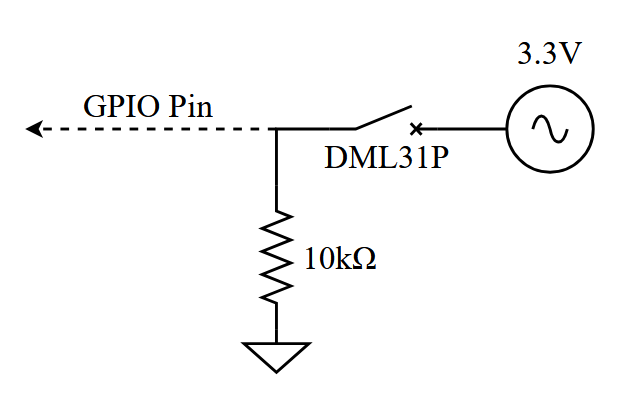
\includegraphics[width=0.5\linewidth]{Figures/endstop-switch-pulldown-circuit.png}
    \caption{End-stop input and pull-down resistor.}
    \label{fig:endstop-switch-pulldown}\label{fig:des-switch}
\end{figure}

\begin{algorithm}[!htbp]
\caption{Debounced end-stop read, called before every major-axis pulse}
\label{alg:gan-endstop}
\begin{algorithmic}[1]
\REQUIRE set of end-stops to ignore (already triggered on this axis)
\FOR{each end-stop not in the ignore set}
    \IF{it does not read closed}
        \STATE \textbf{continue} to the next end-stop
    \ENDIF
    \STATE re-read it twice more, 6\,ms apart \COMMENT{three reads in total, debounce of Equation~\ref{eq:gan-latency}}
    \IF{it read closed on all three reads}
        \STATE \textbf{return} that end-stop as triggered
    \ENDIF
\ENDFOR
\STATE \textbf{return} none triggered
\end{algorithmic}
\end{algorithm}

When an end-stop press is detected, the program enters a stop state by setting both STEP pins low, retracting off every triggered switch and stopping the current gantry task. For the emergency stop to be reset, the end-stop switches must no longer detect contact, for the safety of the system incase the gantry attempts to move further in the direction of the pressed-down switch. A manual force-stop command can also be triggered by the user when the current gantry command must be stopped.

\label{sec:gan-calib}
Calibration is also completed using the end-stop switches. The movement of the gantry depends of the knowledge of its current position to ensure it performs operations in the available movement area of the gantry, but the position after power-up is unknown, so each session begins with a calibration sequence that will automatically reposition the pen starting position to the top-left corner independent of where its existing position was on startup. It will also confirm the available page space that can be drawn on. It drives one way at 1.6\,ms per step until switch of that axis triggers, reverses, and counts the steps $N$ to the \emph{other}. With the hand-measured travel $L$, the resolution, the initial step counter and the position in millimetres are as follows:
\begin{equation}
K_{\mathrm{axis}}=\frac{N}{L},,\qquad x_{\mathrm{mm}}=\frac{n}{K}-5,
\label{eq:des-calibration}
\end{equation}
The 5mm is added for a safe distance away from triggering the end-stop switches accidentally, so the usable area is $190.6\times251.3$\,mm, and each axis retracts 5\,mm off its last switch. Using the nominal 80 microsteps/mm, a 1.6\,ms homing-step period corresponds to 7.8125\,mm/s. Algorithm~\ref{alg:gan-calibrate} states the procedure.

\begin{algorithm}[!htbp]
\caption{Dynamic calibration of one axis}
\label{alg:gan-calibrate}
\begin{algorithmic}[1]
\STATE drive one way at 1.6\,ms per step until either switch of this axis triggers
\STATE reverse; count steps $N$ until the other switch triggers
\STATE $K_{\mathrm{axis}}=N/L$ \COMMENT{$L$ is the hand-measured travel}
\IF{the second switch to trigger was the maximum-side one}
    \STATE $n_0= N$
\ELSE
    \STATE $n_0=0$
\ENDIF
\STATE retract 5\,mm off the switch that is still closed
\IF{an already-triggered switch, an unexpected switch on the other axis, or 200\,000 steps pass with no trigger}
    \STATE abort calibration; refuse all jobs until it is re-run
\ENDIF
\end{algorithmic}
\end{algorithm}

\subsubsection{Gcode generation and motion mapping}
\label{sec:des-drive}
G-code are used to store movement and pen-state commands in a text file. The hardware controller reads each command and its parameters, then converts the coordinates that it must go to into motor pulses. Table~\ref{tab:gcode-command-meanings} describes the commands and parameters used in this projects G-cocde files. The standard G-code commands to travel between coordinates do not include commands to lift or lower the pen. The meanings of \texttt{M3} and \texttt{M5} are the new commands used in this software, where they operate the pen-lift mechanism.

\begin{table}[!htbp]
    \centering
    \begin{tabularx}{\linewidth}{|l|X|}
        \hline
        \textbf{Command or parameter} & \textbf{Meaning in this plotter} \\
        \hline
        \texttt{G21} & Select millimetres as the units for coordinates and feed rates. \\
        \hline
        \texttt{G90} & Use absolute positioning, so each X/Y coordinate is measured from the machine origin. \\
        \hline
        \texttt{G0} & Move rapidly without drawing, used for positioning and travel with the pen raised. \\
        \hline
        \texttt{G1} & Make a straight, feed-controlled move; with the pen down, this draws a line. \\
        \hline
        \texttt{G4 P} & Dwell for the duration specified by P in seconds; used here to let the pen-lift motor finish moving. \\
        \hline
        \texttt{M3} & Lower the pen using the plotter's one-way pen-lift motor. \\
        \hline
        \texttt{M5} & Raise the pen using the plotter's one-way pen-lift motor. \\
        \hline
        \texttt{M2} & End the G-code program. \\
        \hline
        \texttt{X}, \texttt{Y} & Target coordinates in millimetres when used with the active positioning mode. \\
        \hline
        \texttt{F} & Feed rate for movement, in millimetres per minute with \texttt{G21} active. \\
        \hline
        \texttt{P} & Dwell duration in seconds when supplied to \texttt{G4}. \\
        \hline
    \end{tabularx}
    \caption{G-code commands and parameters used in the square-and-triangle test file.}
    \label{tab:gcode-command-meanings}
\end{table}

The following extract shows the G-code commands used to draw a square. Coordinates are in millimetres and use absolute positioning, which means that the pen is lowered before the drawing moves and raised after the square is complete.

\begin{verbatim}
G21
G90
G0 F2400
G0 X45.000 Y76.000
M3
G4 P0.350
G1 F900
G1 X145.000 Y76.000
G1 X145.000 Y176.000
G1 X45.000 Y176.000
G1 X45.000 Y76.000
M5
G4 P0.350
\end{verbatim}

Figure~\ref{fig:gcode-square-triangle-comparison} compares the generated path preview of the generated square, as well as an isometric triangle, with the corresponding physical plot. The test file commands a 100\,mm square and an 80\,mm-base triangle, providing both horizontal and diagonal movements for visual comparison.

\begin{figure}[H]
    \centering
    \begin{minipage}[c]{0.48\linewidth}
        \centering
        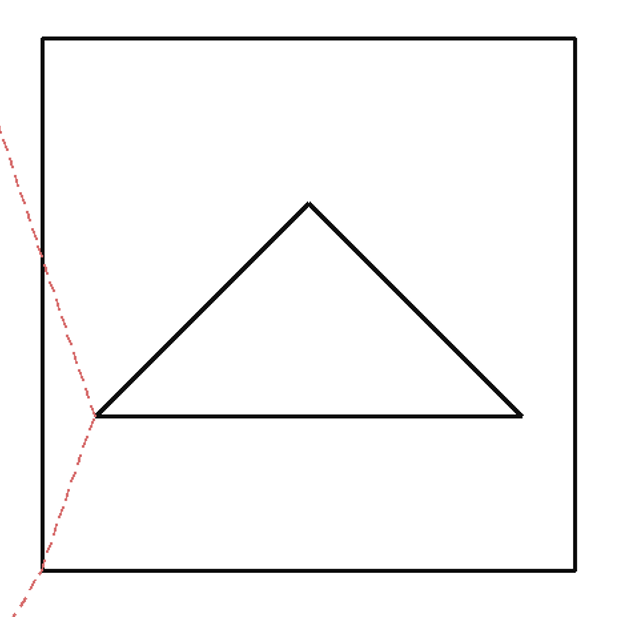
\includegraphics[width=\linewidth,height=0.30\textheight,keepaspectratio]{Figures/square-triangle-gcode-preview.png}\\
        (a) G-code path preview
    \end{minipage}\hfill
    \begin{minipage}[c]{0.48\linewidth}
        \centering
        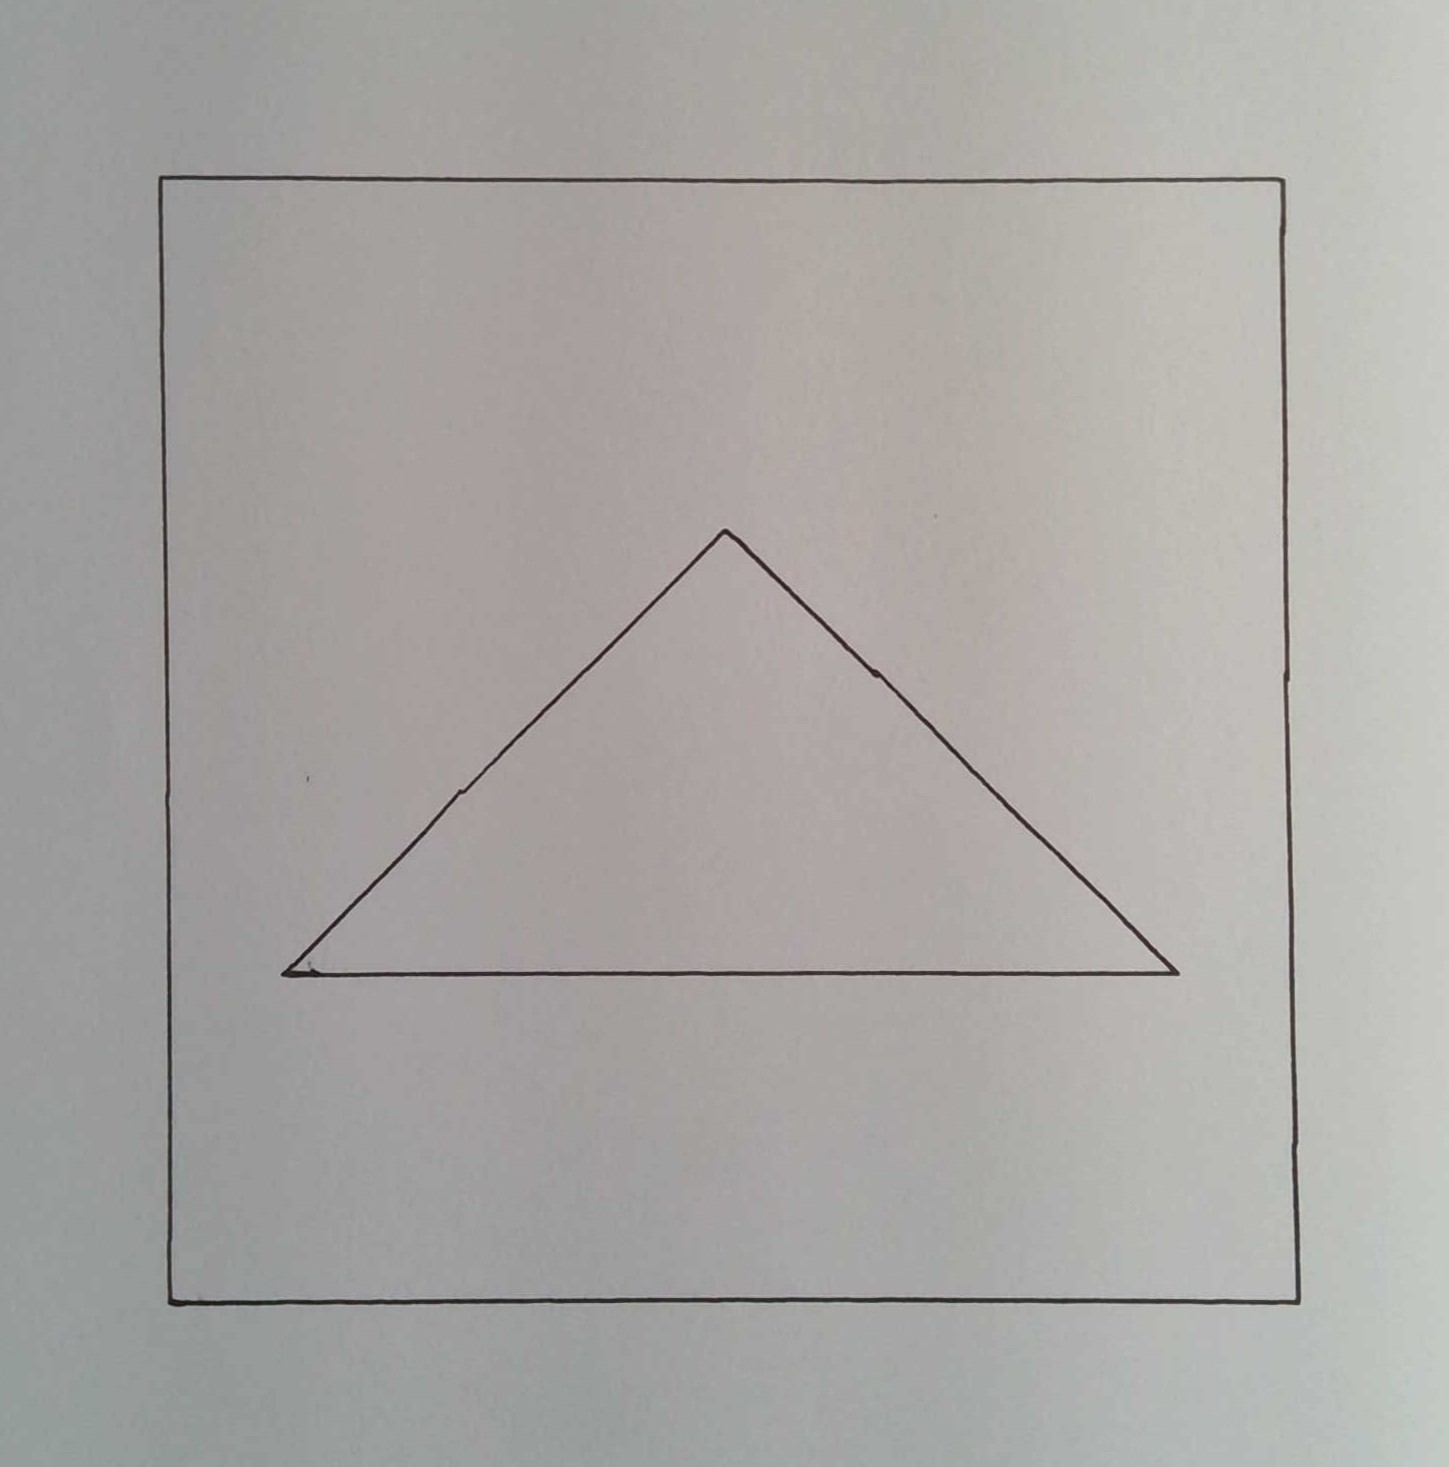
\includegraphics[width=\linewidth,height=0.30\textheight,keepaspectratio]{Figures/square-triangle-reproduced.jpg}\\
        (b) Reproduced drawing
    \end{minipage}
    \caption{Comparison of the G-code preview and the physical square-and-triangle plot.}
    \label{fig:gcode-square-triangle-comparison}\label{fig:des-shapetest}
\end{figure}

\paragraph{Interpolating a straight line.}
Stepping the two axes independently would draw an L-shaped path, so the program interpolates with Bresenham's integer line algorithm~\cite[p.~28]{bresenham1965}, which involves an error term $e$ that is carried along the major axis of $\Delta x$ and $\Delta y$ steps, the major axis is pulsed with a step command every loop, and the minor axis whenever $e$ would go negative. Keeping $e$ in the range of $[0,a_x)$ gives the minor-axis $m_k$ count after $k$ major steps as
\begin{equation}
m_k=\Bigl\lceil\frac{k\,a_y-\lfloor a_x/2\rfloor}{a_x}\Bigr\rceil,
\label{eq:gan-bres}
\end{equation}
Algorithm~\ref{alg:gan-step} states the loop.

\begin{algorithm}[!htbp]
\caption{Coordinated line movement with an integer error accumulator}
\label{alg:gan-step}\label{alg:des-stepping}
\begin{algorithmic}[1]
\REQUIRE signed target changes in microsteps
\STATE set axis directions; choose major count $N_M$ and minor count $N_m$
\STATE $e=\lfloor N_M/2\rfloor$
\FOR{each of the $N_M$ major-axis steps}
    \IF{abort requested or an end-stop is confirmed}
        \STATE \textbf{return} interrupted
    \ENDIF
    \STATE pulse major axis; update its count; $e= e-N_m$
    \IF{$e<0$}
        \STATE pulse minor axis; update its count; $e= e+N_M$
    \ENDIF
\ENDFOR
\end{algorithmic}
\end{algorithm}

Figure~\ref{fig:vt-stepping} Shows a working example of the commanded microsteps for a separate generated move of $(+6,-28)$ microsteps. Its highest difference from the ideal line is 0.5 microsteps, or $0.5/80=0.00625$\,mm. This plot shows how the major axis gets pulsed every iteration (the y microsteps), while the error adds up in the minor axis and steps when the error gets too large (the x microsteps)
\begin{figure}[H]\centering
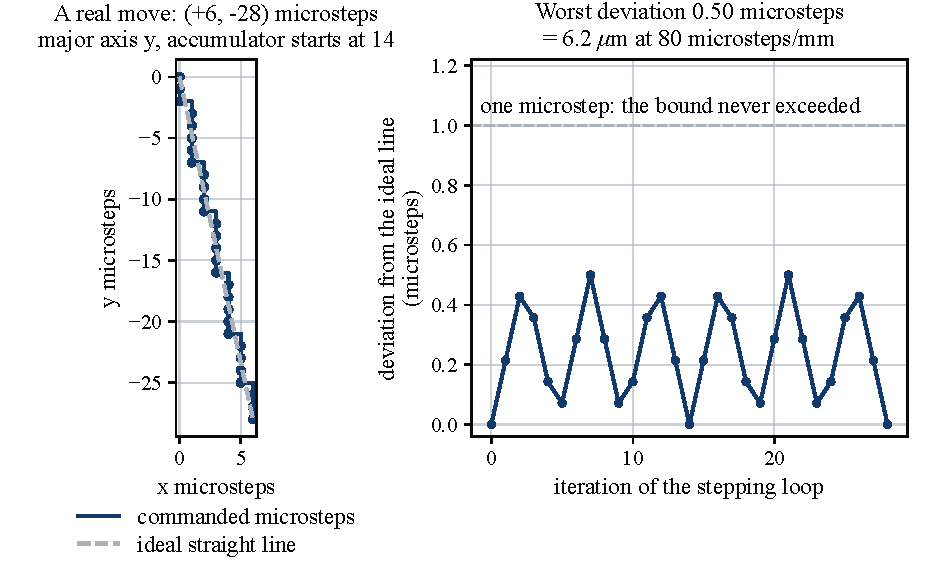
\includegraphics[width=0.96\linewidth]{Figures/VisualTests/T52_bresenham_staircase.pdf}
\caption{Integer axis stepping and command-space deviation for a generated move.}
\label{fig:vt-stepping}
\end{figure}
